\documentclass[12pt]{article}
\usepackage{style}

\begin{document}

\section{Abstract}
We are making an Andriod application for the company Ebogreolen.dk. This application needs features that enables their customers to search for e-books or audiobooks. The application should make the users able to buy e-book and audiobooks. This means that there needs to be a payment method for the e-books and audiobooks as well. Additional features, if possible, would be to implement a way of reading or hearing the e-books or audiobooks thought this is not a requirement for the finished product.\\
This is done in the group with meetings each week where we discuss what subjects should be completed in near future and what subjects that can wait until later. These tasks are fullfilled in get togethers on weekends and weekdays if needed. The article specifies how far we are in development, how the group work is goin and the progress in general.\\
\\
This article discusses the project as a whole. More specifically, the functional requirements of the project described with different diagrams. It discusses the user interface with screens of the user interface as well as a description of the interaction between the user and the application.

\section{Userinterface and interaction design}
\subsection{Userinterface and userinteraction}

The external interfaces are here understood as the finished product GUI, for which we have a course outline as it follows in Figure \ref{Front page},\ref{Book information},\ref{Categories} and \ref{Results}. The application GUI for the login page has not been developed yet.
\begin{SCfigure}
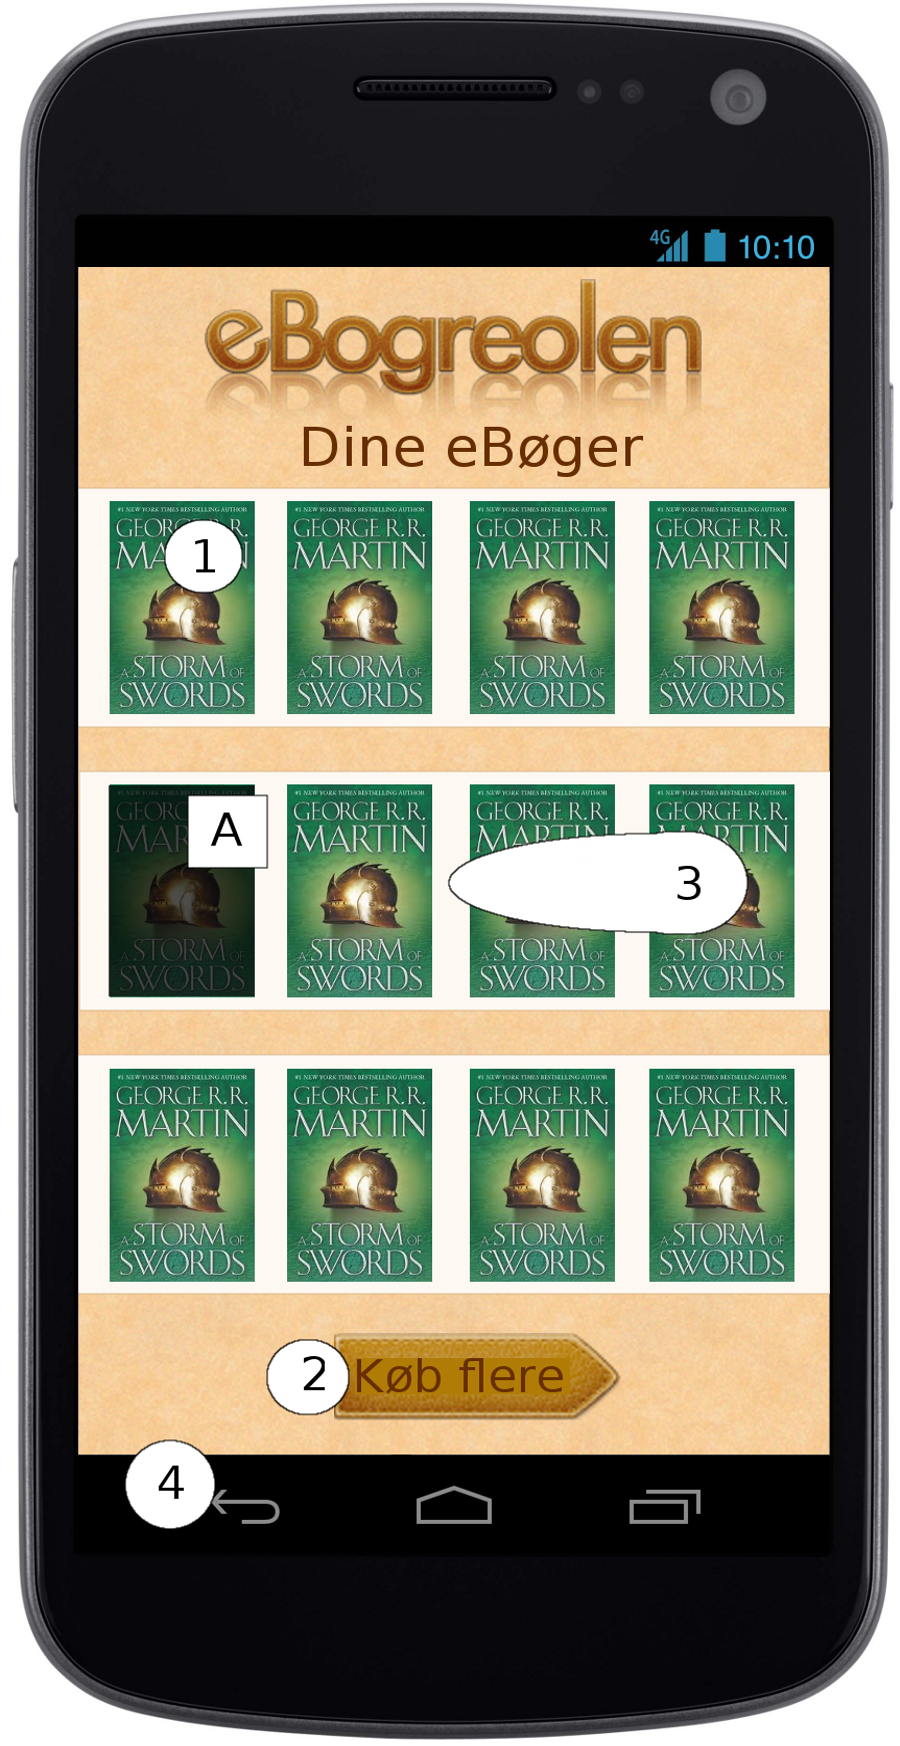
\includegraphics[scale=0.7]{gnexforside.png}
\caption{
\\
1. Open a page containing the information of a purchased book, this will lead to Figure \ref{Book information}.\\\\
2. Search/browse after more books to purchase, this will lead to Figure \ref{Categories}.\\\\
3. Swipe to the side to look at more of your books.\\\\
4. This button will always go one page back, if there are no more pages to go back, the application will be closed.\\\\\\
A. This book is darkened, because the book has been purchased, but not downloaded.
}
\label{Front page}
\end{SCfigure}

\begin{SCfigure}
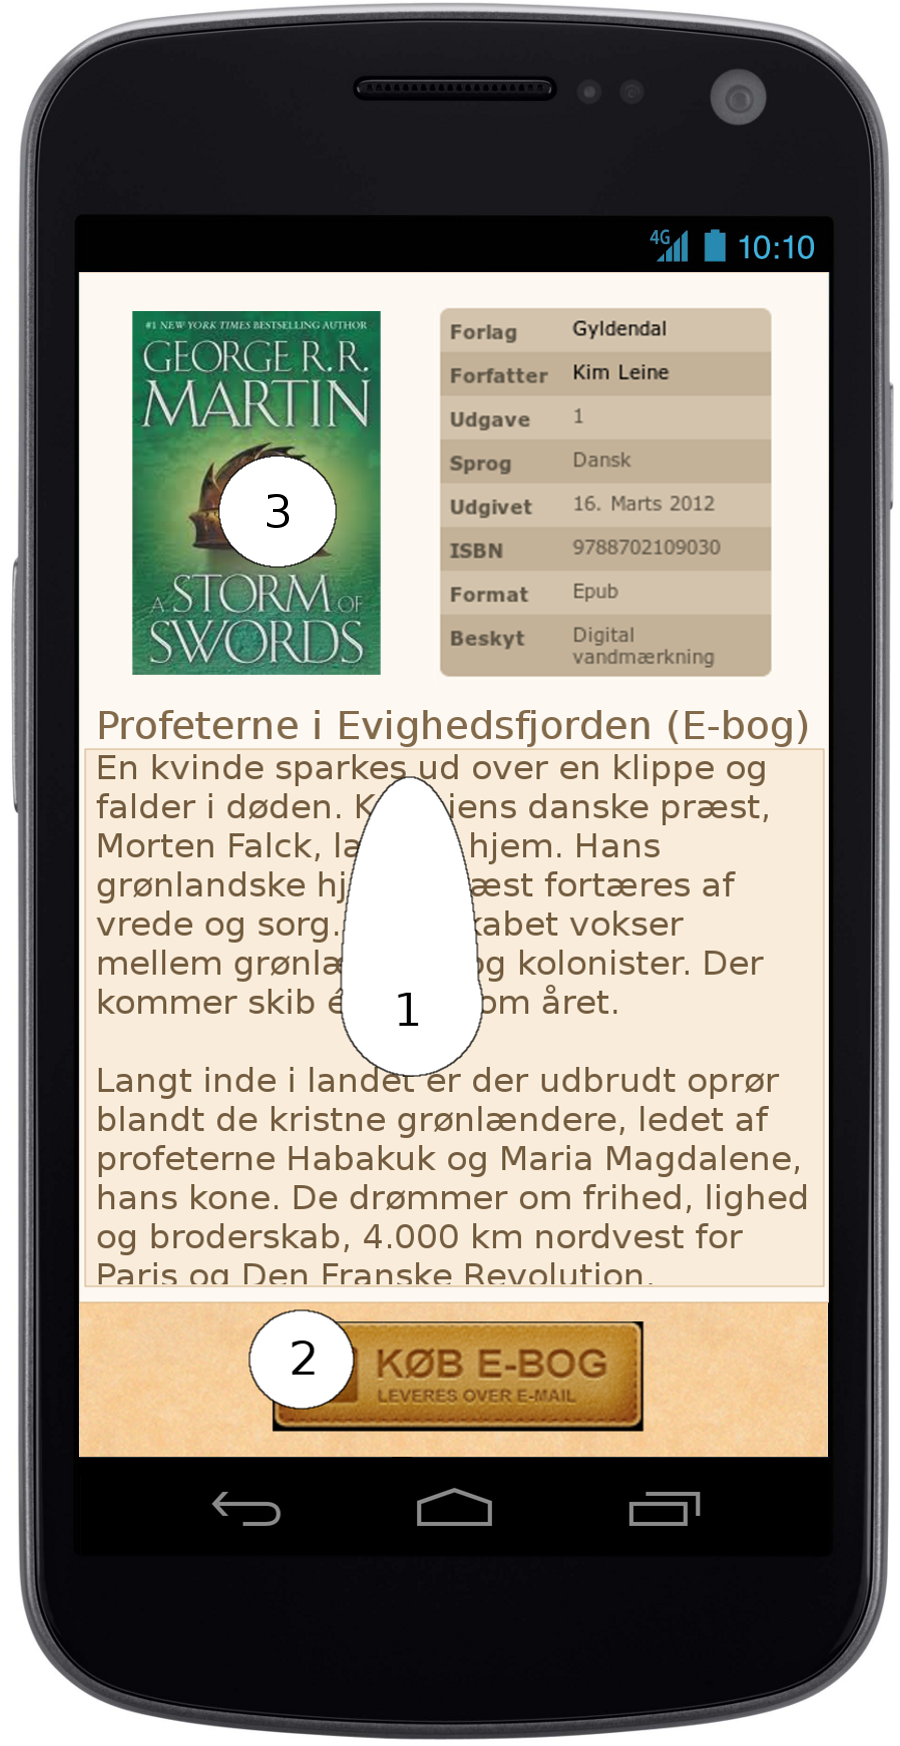
\includegraphics[scale=0.7]{gnexinfodownloadogkoeb.png}
\caption{
\\
1. Swipe up and down to read a description of the book.\\\\
2. This button can be a: Buy, Download, Read or Listen button, this depends on whether or not you own the material and/or if its an audiobook or ebook.\\\\
3. By pressing here, a larger image of the books cover.
}
\label{Book information}
\end{SCfigure}
\begin{SCfigure}
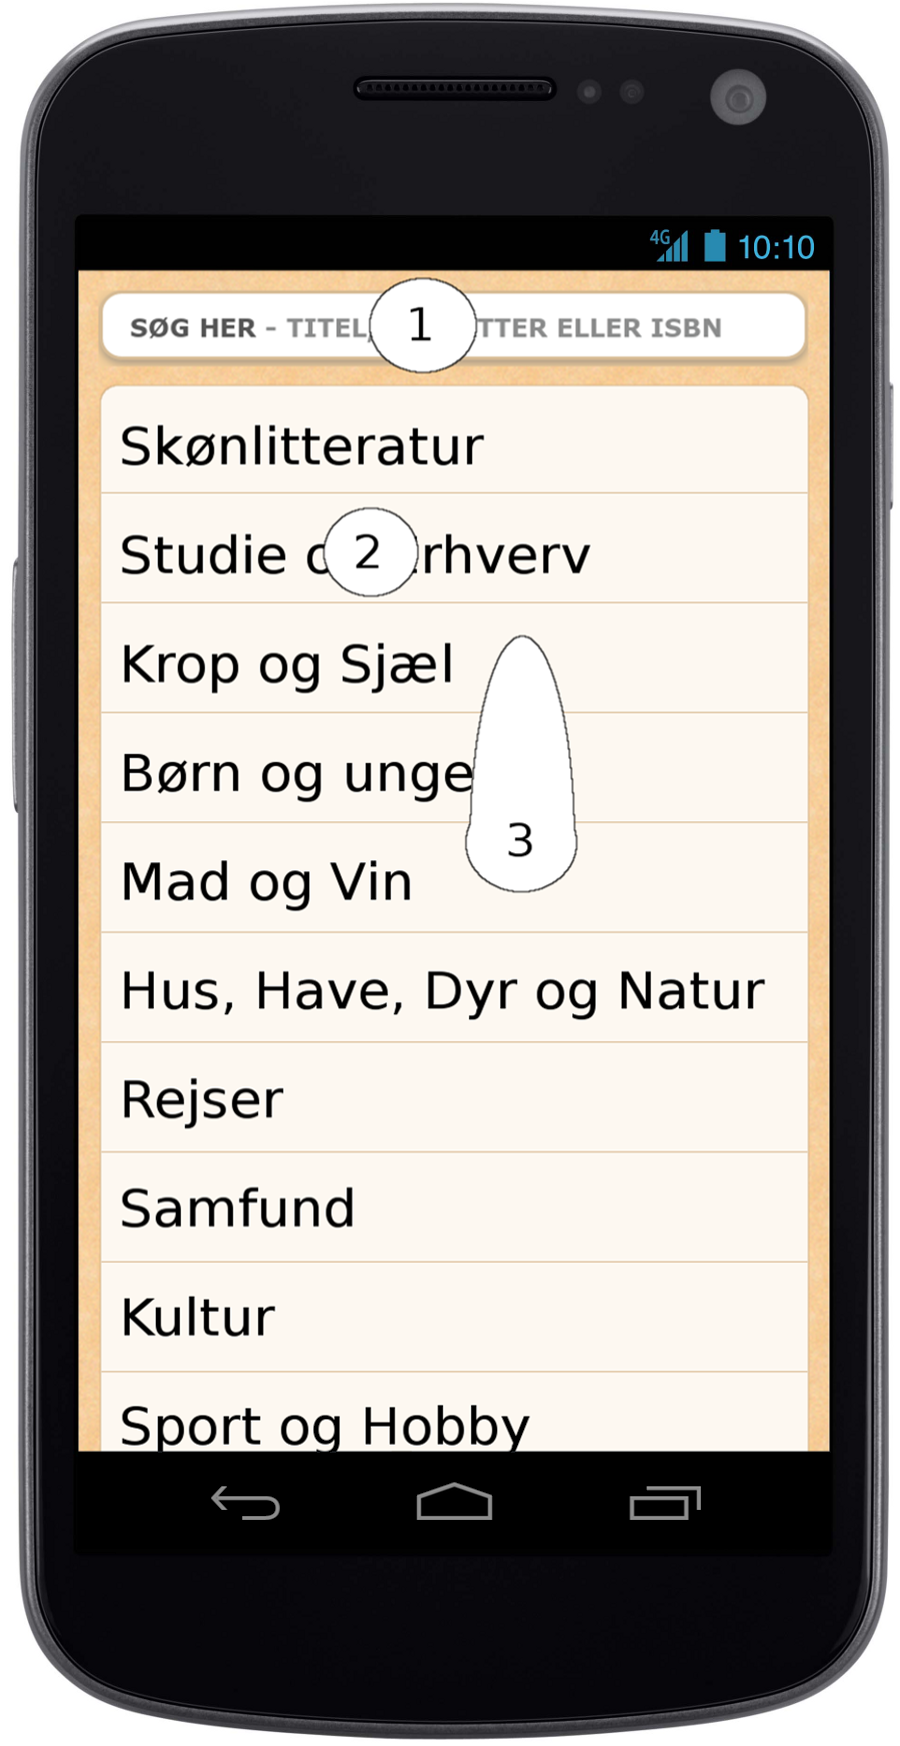
\includegraphics[scale=0.7]{gnexsoegeogbrowse.png}
\caption{
\\
1. This will access the search function, when a search is complete it will direct you to Figure \ref{Results}\\\\
2. The will open the category in this interface if it is a super category, and go to Figure \ref{Results} it is a sub category.\\\\
3. Swipe up and down to browse the categories.
}
\label{Categories}
\end{SCfigure}

\begin{SCfigure}
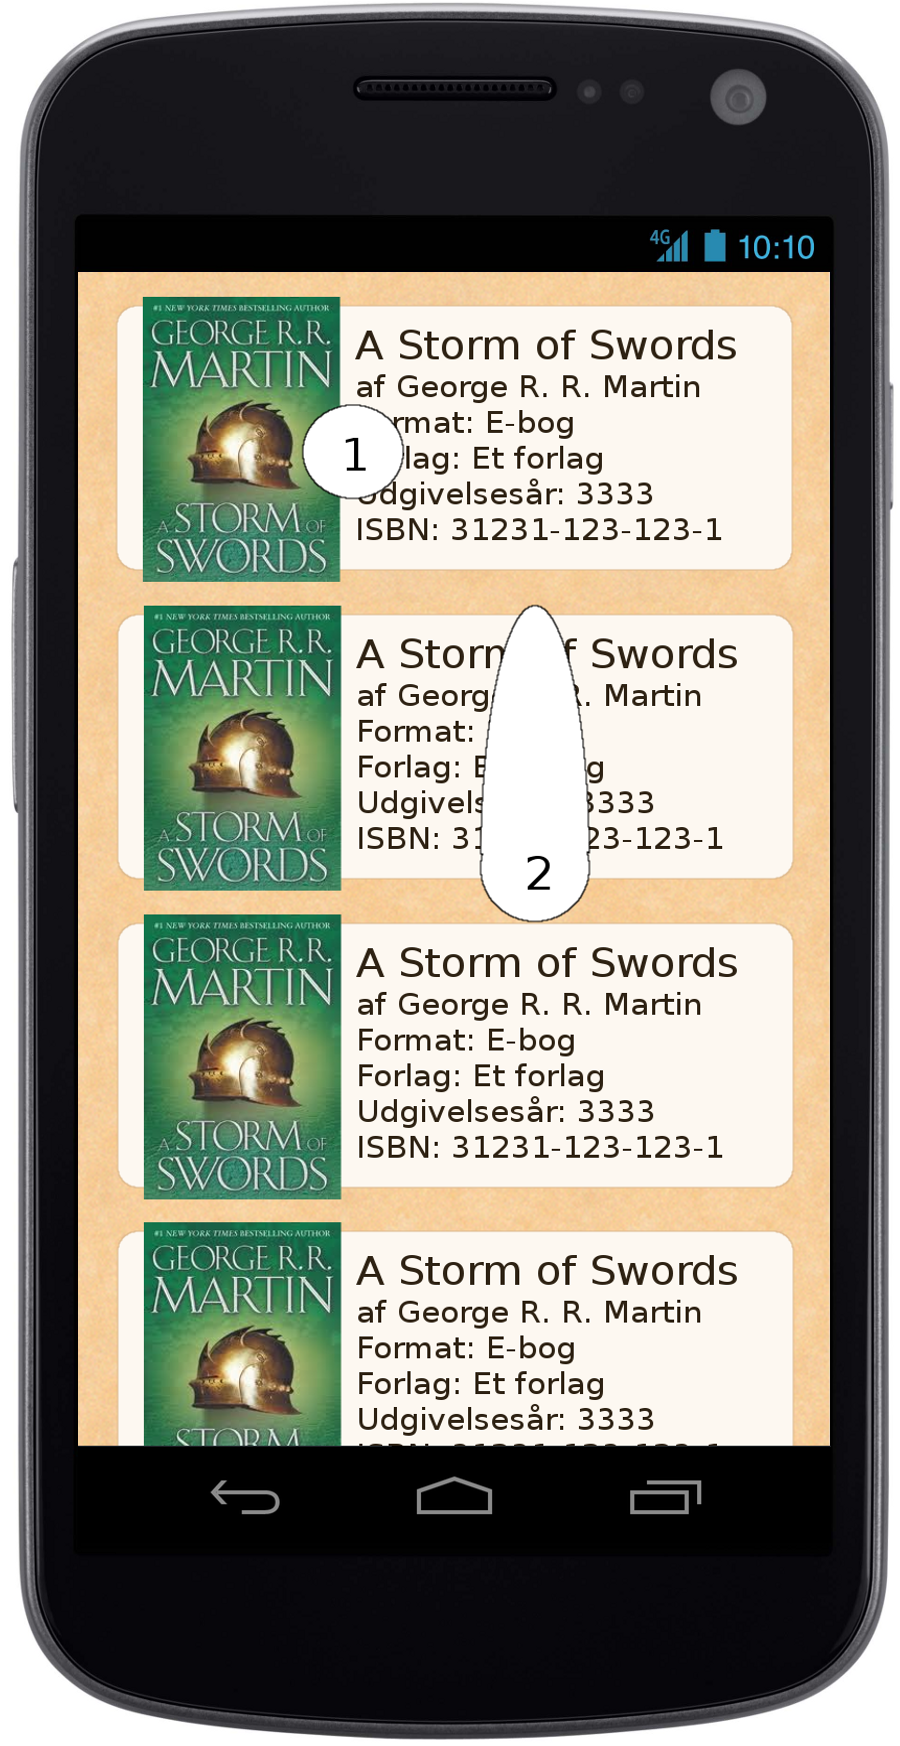
\includegraphics[scale=0.7]{gnexresultater.png}
\caption{
\\
1. This will take you to the information of the given book, this will lead to Figure \ref{Book information}.\\\\
2. Swipe up and down to browse the results.
}
\label{Results}
\end{SCfigure}

\subsection{Audio-visual presentation}
On this stage we do not have a prototype of our product, but the final product is exptected to look like what's given in section 6.1

\subsection{d}
 

\section{Project collaboration}
We have developted a 'game' using "experience' points and the oppotunity to 'level' up. These point are distributed to the group participants by a point generator on:
$$LINK PLOX$$
that generates a random amount of point in a certain range. The range is calculated from tasks completed. Tasks are worth points equal to the hours of work estimated during our scrum and these translates into points that provides the range from your random gain of experience.\\
The experience needed to level up increases each time using the fibonacci sequence.\\
This game a motivation for us since there are small benefits (bragging rights, beers etc) and the idea of making it competitive is appealing to all of us. While keeping the simple benefits, it won't ruin the dynamics in the group. Keeping it on a low level, a fun sidekick, we keep the ambitions and motivation high while still maintaining our good teamwork.

\end{document}